% ----------------------------------------------------------
\chapter{Fundamentação}\label{cap:fundamentacao}
% ----------------------------------------------------------


% ----------------------------------------------------------
\section{Normas e Padrões de Testes}\label{sec:normas-ecss}
% ----------------------------------------------------------
% TODO: Pensar num nome melhor para esta parte

A principal referência a ser seguida em uma missão envolvendo CubeSats é o CubeSat Design Specification, ou \gls{CDS} \cite{cds}, que é o documento que define as especificações do padrão CubeSat.

Além do \gls{CDS}, recentemente, tem-se exemplos de missões de CubeSat seguindo os padrões e normas da \gls{ECSS}, como \textcite{floripasat-1}, \textcite{tailoring-ecss-nanosat} e \textcite{mist-eps}, tanto para etapa de testes quanto para desenvolvimento da missão como um todo.

Ambas estas referências introduzem conceitos e requisitos relevântes à elaboração de um plano de testes que serão apresentados a seguir.

% ==== CubeSat Design Specification ====
\subsection{CubeSat Design Specification}

O \gls{CDS} é um documento contendo as especificações e requisitos basicos e servindo como ponto de partida para o design de CubeSats de 1U a 12U, mantido pela California Polytechnic State University.
Requisitos gerais, mecanicos, elétricos, de operação ede testes são especificados, definindo as características básicas que constituem um nanosatélite da classe CubeSat.

Os requisitos de testes descritos no \gls{CDS} estão focados em testes ambientais para o CubeSat como um todo, já em estagio de qualificação para o lançamento.
Como filosofia de testes, o \gls{CDS} propõe as seguintes etapas: \textit{qualification}, \textit{acceptance} e \textit{proto-flight}, executadas conforme o diagrama mostrado na \autoref{fig:test-flow-cds}.

% Fluxograma de testes do CDS
\begin{figure}[htp]
    \caption{Fluxo de testes geral de um CubeSat}
    \begin{center}
        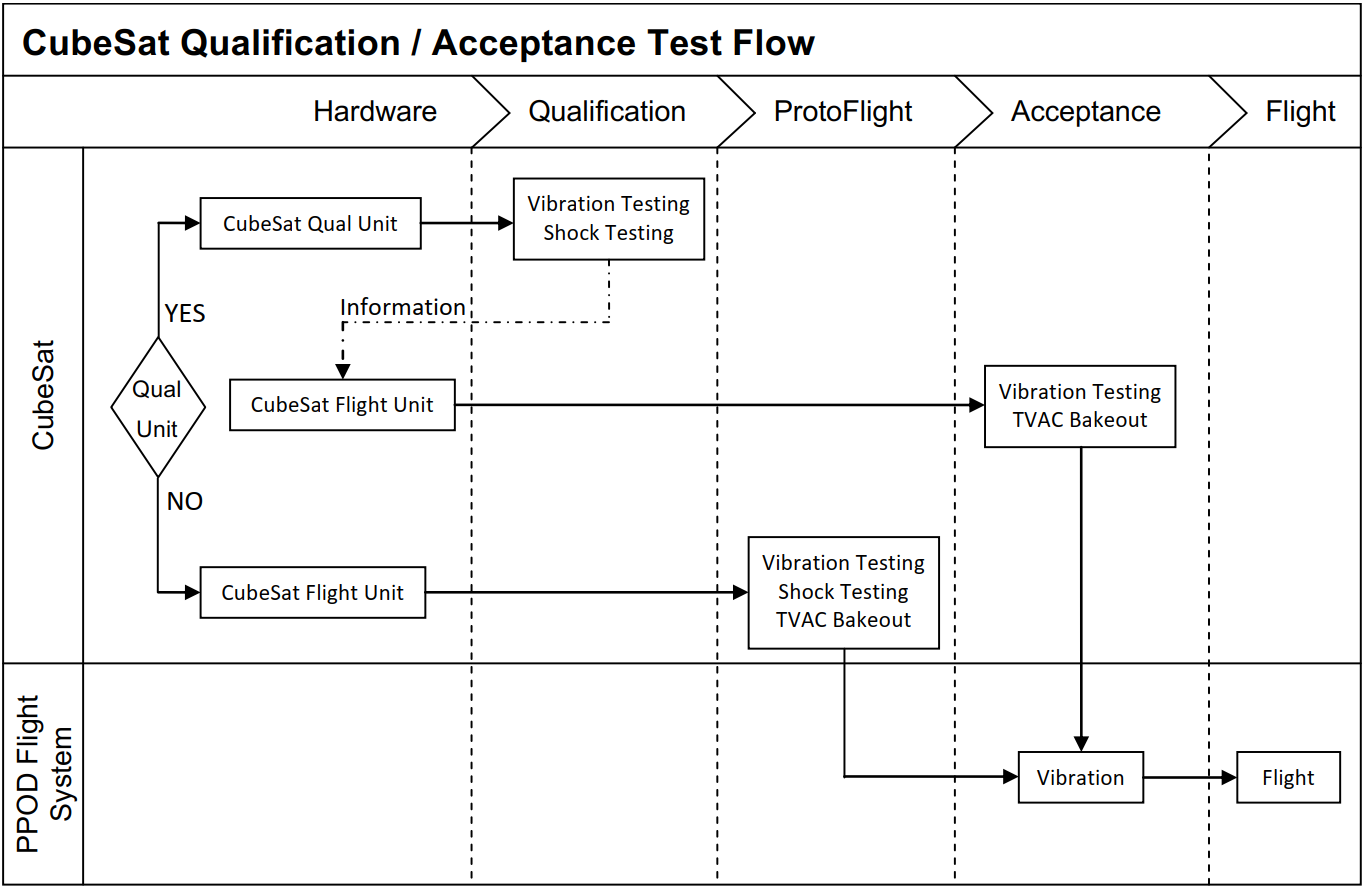
\includegraphics[width=\textwidth, keepaspectratio]{images/test-flow-diagram-cds.png}
    \end{center}
    \fonte{\textcite{cds}.}
    \label{fig:test-flow-cds}
\end{figure}

Os principais testes indicados pelo \gls{CDS} são:
\begin{itemize}
    \item Testes de vibração;
    \item Termo vácuo e bakeout;
    \item Testes de choque;
    \item Inspeção visual;
\end{itemize}

É importante ressaltar que estes requisitos de teste, bem como os parâmetros (intencidade, duração, etc...) de cada teste para cada etapa, como enfatizado no próprio documento, são apenas preliminares e servem somente como base. Os requisitos de teste oficiais para lançamento serão gerados pelo provedor do lançamento, e sempre tomarão precedência em relação aos requisitos do \gls{CDS} ou a qualquer outro conjunto de requisitos.


% ==== European Cooperation For Space Standardization ====
\subsection{European Cooperation for Space Standardization}

A European Cooperation for Space Standardization, ou \gls{ECSS}, é uma colaboração entre a \gls{ESA}, a indústria espacial europeia e diversas outras agências espaciais, responsavel por desenvolver e manter um conjunto de normas e padrões relacionados a atividades espaciais. Essas normas e padrões cobrem diversas disciplinas, como gerenciamento, engenharia, controle de qualidade e sustentabilidade.

Dentro do ramo de engenharia, tem-se os documentos ECSS-E-ST-10-02 \cite{ecss-e-st-10-02}, ECSS-E-HB-10-02 \cite{ecss-e-hb-10-02}, ECSS-E-ST-10-03 \cite{ecss-e-st-10-03} e ECSS-E-HB-10-03 \cite{ecss-e-hb-10-03}, que determinam requisitos para os processos de verificação e testes. Estes documentos são redigidos de forma genérica, com o objetivo de que, a partir de um processo de tailoring, possa-se aplicar estas normas e padrões em diversos níveis, tando ao satélite completo quanto a um módulo isoladamente.
Como complemento às normas ECSS-E-ST-10-02 e ECSS-E-ST-10-03, tem-se tabmém o documento ECSS-S-ST-00-01 \cite{ecss-s-st-00-01}, um glossário onde diversos termos e definições utilizados nas demais normas são apresentados.
Vale ressaltar também que estes documentos não são específicos para nanosatélites, mas foram pensados para satélites de médio e grande porte, onde se necessita uma rigorosidade extrema nos processos de \gls{AIV}.
Portanto deve-se levar em consideração o cenário de uma missão de CubeSat e fazer as adaptações necessárias ao se aplicar estas normas, especialmente em uma missão universitária, visando simplicidade, baixo custo e rápido desenvolvimento.

De acordo com as normas citadas acima, testes são considerados como um dos métodos utilizados para o processo de verificação.
Com isso, apesar deste trabalho ser focado em testes, alguns conceitos relacionados ao processo de verificação, introduzidos em \cite{ecss-e-st-10-02}, como \textit{verification levels}, \textit{verification stages} e \textit{model philosophy}, influenciam diretamente nos objetivos e na elaboração do plano de testes.

Similarmente à filosofia de testes apresentada pelo \gls{CDS}, em \textcite{ecss-e-st-10-03} tem-se os conceitos de \textit{qualification testing}, \textit{acceptance testing} e \textit{proto-flight testing}, que determinam os objetivos do plano de testes.

\subsubsection*{\textit{Verification Levels}}

Os níveis de verificação estão relacionados à decomposição do produto final, neste caso um CubeSat. Estes níveis podem varias de acordo com a complexidade do projeto.
Os níveis de decomposição típicos são mostrados no anexo B.1 de \textcite{ecss-s-st-00-01}.

O processo de verificação é executado em cada um dos níveis definidos para um projeto ou missão.

\subsubsection*{\textit{Verification Stages}}

O processo de verificação é feito em estágios, com objetivos específicos. Os principais estágios apresentados em \textcite{ecss-e-st-10-02} são \textit{qualification}, \textit{acceptance}\red{, \textit{pre-launch}, \textit{in-orbit}, e \textit{post-landing}}.
\red{Falar de todos os estágios aqui ou já selecionar apenas os aplicáveis à CubeSats  e módulos EPS?}

O estágio de \textit{qualification} visa garantir que o design proposto para a missão é capaz de cumprir com os requisitos no ambiente esperado.

O estágio de \textit{acceptance} visa demostrar que o modelo final \red{modelo físico de vôo} está em conformidade com o design qualificado préviamente


\subsubsection*{\textit{Model Philosophy}}

O conceito de \textit{model philosophy} está relacionado ao tipo e quantidade de modelos físicos utilizados durante o desenvolmento, verificação e testes.

Em \cite{ecss-e-hb-10-02}, diversos tipos de modelos são apresentados e descritos. Considerando uma missão de CubeSat, os principais modelos aplicaveis são: modelo de engenharia, modelo de qualificação, modelo de proto-flight e modelo de vôo.
\red{Descrever os modelos?}


\subsubsection*{\textit{Qualification Testing}}

Testes de qualificação (chamado \textit{qualification testing} na ECSS-E-ST-10-03) tem o objetivo de verificar que o design do objeto sobre teste é capaz de satifazer todos os seu requisitos. Estes testes são conduzidos em modelos de qualificação dedicados e com parâmetros de teste (intesidade, duração) específicos.


\subsubsection*{\textit{Acceptance Testing}}

Testes de aceitação (chamado \textit{qualification testing} na ECSS-E-ST-10-03) tem o objetivo de verificar que o objeto sobre teste está em conformidade com o design que foi qualificado préviamente e se encontra livre de defeitos de fabricação. Estes testes são conduzidos em todos os modelos de vôo e com parâmetros de teste (intesidade, duração) específicos para \textit{acceptance testing}.


\subsubsection*{\textit{Proto-Flight Testing}}

Testes de proto-flight (chamado \textit{proto-flight testing} na ECSS-E-ST-10-03) podem ser executados no primeiro modelo de vôo e combinam os objetivos dos testes de qualificação e aceitação. Os parâmetros de teste (intesidade, duração) utilizam as intensidades definidas para qualificação com as durações definidas para aceitação.



% ----------------------------------------------------------
\section{Topologias e arquiteturas de EPS}\label{sec:arq-top}
% ----------------------------------------------------------

Nesta seção serão apresentadas diferentes topologias e arquiteturas de \gls{EPS} para CubeSats com o intuito de identificar os principais aspectos e características relevantes para a criação de um plano de testes.

Neste trabalho, topologia se refere a uma visão de alto-nível dos principais blocos funcionais do sistema e arquitetura se refere ao modo como uma dada topologia é implementada.

% ----------------------------------------------------------
\subsection{Topologias}\label{sec:topologias}
% ----------------------------------------------------------

Um módulo \gls{EPS} é composto por algum elementos básicos, mostrados na \red{Figura X}.
O sistema de harvesting é responsável por extrair energia dos painéis solares, que sã oa fonte primaria de energia dos CubeSats.
O sistema de armazenamento de energia é utilizado para alimentar o satélite em períodos de eclipse ou em situações de alta demanda de energia.
O sistema de distribuição é responsável por entregar a energia coletada e armazenada pelo \gls{EPS} de forma adequada às cargas.
Cargas típicas de um \gls{EPS} envolvem desde os módulos de serviço, como \gls{OBDH} e \gls{TTC}, quanto cargas úteis que variam conforme os objetivos de cada missão.
O barramento que interliga estes elementos, no contexto deste trabalho, será chamado de barramento principal.


O estudo de \textcite{comprehensive-review-eps} mostra uma revisão de diferentes topologias de \gls{EPS} utilizados em diversas missões e propõe uma forma de classificalos de acordo com quatro aspectos principais em comum nas diversas topologias:
\begin{itemize}
    \item Estágios de conversão;
    \item Tipo de distribuição; % Localização dos conversores ods barramentos de saída
    \item Tipo de sistema de harvesting;% Sistema de harvesting
    \item Regulação do barramento principal;% Nome melhor para este barramento
\end{itemize}

Estágios de conversão refere-se à quantidade de conversões de energia realizadas até que a energia dos painéis ou baterias seja entregue às cargas. Até o momento, encontram-se em publicações ou patentes apenas topologias com múltiplos estágios de conversão para \gls{EPS}s de CubeSats \cite{comprehensive-review-eps}.

Em relação à localização dos conversores dos barrametos de saída, tem-se topologias centralizadas, com os conversores localizados num mesmo local ou na mesma PCB, ou distribuida, com os conversores localizados em diferentes locais ou PCB com o intuito de estarem fisicamente mais próximos às cargas.

Em relação ao tipo de sistema de harvesting, que realiza a interface com os painéis solares, tem-se topologias com \gls{DET}, onde os painéis são conectados diretamente ao sistema de armazenamento e/ou aos reguladores das cargas, ou topologias com \gls{PPT}, onde os painéis são conectados à conversores dc-dc operados de forma a realizar \gls{MPPT}.
Adicionalmente, no estudo de \textcite{sara-review-eps}, diferenciam-se entre utilização de conversores discretos ou via circuitos integrados, e também apresenta-se a utlização de reguladores VLDO para interfacear com os painéis solares.

Em relação à regulação do barramento principal, tem-se topologias com barramento principal regulado, onde há um conversor regulando o mesmo para uma tensão de referência, não-regulado, onde os terminais da bateria são conectados diretamente ao barramento, ou parcialmente regulado, em que o barramento é regulado apenas durante o periodo iluminado da orbita.



% ----------------------------------------------------------
\subsection{Arquiteturas}\label{sec:arquiteturas}
% ----------------------------------------------------------

A seguir serão analizadas as arquiteturas de diferentes modelos de \gls{EPS}, tanto de desenvolvimento próprio quanto modelos comerciais, a fim de identificar aspectos e características em comum relevantes para o desenvolvimento do plano de testes.

%  ==== Aalto-2 EPS ====
\subsubsection{Aalto-2 EPS}

O \gls{EPS} desenvolvido para o satélite Aalto-2, descrito em \textcite{aalto-eps}, utiliza uma topologia de distribuição centralizada, conversão multiestágio, sistema de harvesting com \gls{PPT} e barramento principal não regulado.
Além disso, possui um microcontrolador MSP430 para controle e monitoramento e redundâncias em hardware para as funcionalidades principais como conversores DC-DC, reguladores de carga de bateria e \gls{MPPT}.

O sistema de harvesting deste \gls{EPS} possui dois canais com CIs dedicados para a realização de \gls{MPPT}. O conjunto de painéis solares de cada eixo, X e Y, é ligado ao barramento principal através de um \gls{BCR}, neste caso o LT3652.

Para armazenamento de energia o EPS do Aalto-2 utilizará duas células de baterias em paralelo (configuração 1s2p). O modelo das baterias ainda não havia sido determinado, porém a inclusão de circuitos de proteção contra over-charge e over-discharge, assim como a necessidade de um sistema de aquecimento para as baterias já estavam previstos.

O sistema de distribuição consiste em dois barramentos, de 3.3V e 5V, utilizando os reguladores LTC1875 e LTC3122 respectivamente.
Cada barramento possui reguladores duplicados em redundância fria.
Possui também um barramento dedicado para alimentar o microcontrolador.
Para controle dos barramentos foram utilizados MOSFETs MAX890L, que além de atuarem como chaves, possuem limitação de corrente proporcionando proteção contra over-current.
Além disso, corrente e tensão nos barramentos são monitoradas pelo microcontrolador.

Para controle e monitoramento, foi utilizado o microcontrolador MSP430-F1611. Tensões, correntes e temperaturas são medidas através do CI LTC2991. Os seguintes dados de telemetria são monitorados e transmitidos ao computador de bordo pelo EPS:
\begin{itemize}
    \item Tensões, correntes e temperaturas dos painéis solares.
    \item Tensões, correntes e temperatuas de cada célula das baterias.
    \item Status de carga das baterias.
    \item Tensões e correntes nos barramentos de saída do EPS.
\end{itemize}


%  ==== ESTCube-1 EPS ====
\subsubsection{ESTCube-1}

O \gls{EPS} desenvolvido para o satélite ESTCube-1, descrito em \textcite{estcube-eps}, utiliza uma topologia de distribuição centralizada, conversão multiestágio, sistema de harvesting com \gls{PPT} e barramento principal não regulado.
Possui também um microcontrolador para controle e monitoramento e inclui redundâncias em hardware.

O sistema de harvesting é composto por três canais de \gls{MPPT}. Cada canal utiliza um chip SPV1040 para a realizar o \gls{MPPT} de um conjunto de painéis correspondente a um dos eixos do satélite.

Duas células de bateria de íon de lítio são utilizadas para armazenamento, com monitoramento de tensão, corrente e temperatura. Cada célula é conectada ao barramento principal através de duas chaves de potência TPS2557, controlando as direções de carga e descarga separadamente e servindo como proteção.

O sistema de distribuição é composto por três barramentos, 3.3V, 5V e 12V, utilizando os reguladores LTC3440 para os barramentos de 3.3V e 5V, e LM2700 para o barramento de 12V.
Cada barramento possui os conversores duplicados em redundância quente.
O microcontrolador e outros circuitos do \gls{EPS} são alimentados por um barramento secudário dedicado.
Os barramentos possuem também chaves de potência, TPS2551 ou TPS2557, com proteção contra over-current, que conectam os reguladores tanto ao barramento principal quanto aos barramentos de saída.

O controle deste \gls{EPS} é realizado por um microcontrolador ATMega1280 e utiliza de memórias FRAM para armazenamento do firmware, variáveis de controle e variáveis de estado.
Comunicação com os outros módulos do satélite é feita via \gls{UART}.
O monitoramento é ralizado através de 44 sensores de tensão e corrente em diversos pontos do sistema e um conjunto de ADCs dedicados, além ADC interno do microcontrolador.

Este \gls{EPS} é responsável por realizar os procedimentos de inicialização do satélite pós lançamento e também por controlar o rádio de transmissão do beacon.




%  ==== MIST EPS ====
\subsubsection{GomSpace NanoPower P31u e BP4}

O NanoPower P31u \cite{p31u-datasheet} é um modelo comercial de \gls{EPS} fabricado pela empresa GomSpace. Utiliza uma topologia de distribuição centralizada, conversão multiestágio, sistema de harvesting com \gls{PPT} e barramento principal não regulado. Possui também um microcontrolador para controle, configuração e comunicação.

O sistema de harvesting consite de três canais com conversores para realização de \gls{MPPT}, controlados pelo microcontrolador.

O sistema de distribuição utiliza de dois barramentos regulados, de 3.3V e 5V, e seis canais de saída controlados por chaves de potência com limitação de corrente, configuraveis individualmente para 3.3V ou 5V.

Um microcontrolador é responsável pelo gerenciamento do \gls{EPS} e o comportamento pode ser configurado pelo usuário via interface \gls{I2C}.
Dentre as funcionalidades tem-se: modo de operação do \gls{MPPT}, acesso aos logs de tensões, correntes e temperaturas em diversos pontos do sistema, acionamento de aquecedor de baterias, controle dos canais de saída.

Este EPS é comumente utilizado em conjunto com o módulo de baterias NanoPower BP4 \cite{bp4-datasheet}, que é uma das opções de armazenamento oferecidas pela empresa GomSpace.
Este módulo utiliza quatro células de baterias de íon de lítio configuradas em 2s-2p ou 4s-1p. Possui sensores de temperatura com interface digital e aquecedor para as baterias.



%  ==== EPS 2.0 ====
\subsubsection{EPS 2.0}

O \gls{EPS2} é a segunda geração de módulo \gls{EPS} projetado para a plataforma multi-missão desenvolvida no SpaceLab, será utilizado nas missões GOLDS-UFSC e Constelação Catarina e encontra-se nos estágios finais de desenvolvimento. Este \gls{EPS} é uma evolução direta do módulo utilizado no FloripaSat-1 \cite{floripasat-1}. A documentação do \gls{EPS2} pode ser encontrada em \cite{eps2-doc}, a \autoref{fig:eps2-diagrama-blocos} mostra o diagrama de blocos deste sistema.

% Diagrama de blocos do EPS 2.0
\begin{figure}[htp]
    \caption{Diagrama de blocos do EPS 2.0}
    \begin{center}
        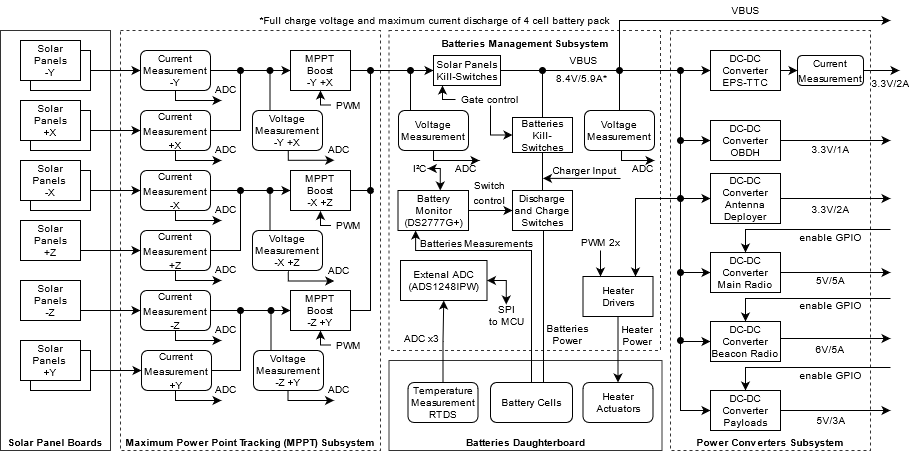
\includegraphics[width=\textwidth, keepaspectratio]{images/eps2-power-diagram.png}
    \end{center}
    \fonte{\textcite{eps2-doc}.}
    \label{fig:eps2-diagrama-blocos}
\end{figure}

Este módulo implementa uma topologia de distribuição centralizada, com múltiplos estágios de conversão, sistema de harvesting com \gls{PPT} e barramento principal não regulado.
Possui também um microcontrolador para operação, leitura de sensores e comunicação cos os demais módulos do satélite.

O sistema de harvesting consiste em três canais com conversores boost discretos e sensores de tensão e corrente, controlados individualmente pelo microcontrolador para realizar \gls{MPPT}, utilizando o algorítimo de \gls{PO}.

O sistema de distribuição consiste em seis barramentos com conversores dedicados, de 3.3V, 5V ou 6V, para cada um dos módulos do satélite, que podem ser atviados ou desativados individualmente.

O sistema de armazenamento consiste de um sistema de monitoramento (chamado \textit{Batteries Management Subsystem} na \autoref{fig:eps2-diagrama-blocos}) e de um módulo de baterias separado (chamado \textit{Batteries Daughterboard} no diagrama da \autoref{fig:eps2-diagrama-blocos}), que pode ser acoplado ao \gls{EPS2}.
O módulo de baterias contem 4 células de baterias de íon de lítio em configuração 2s-2p, bem como sensores de temperatura e aquecedores que podem ser lidos e controlados pelo microcontrolador do \gls{EPS}.
O sistema de monitoramento é ralizado pelo CI DS2777G+, que realiza leituras de tensão e corrente das baterias, proteção contra over-charge e over-discharge, estimativas de vida útil e monitoramento do estado de carga das baterias.
Os sensores de temperatura são lidos por um conversor AD dedicado ADS1248 e utilizados para controle dos aquecedores de bateria, os driver para acionamento dos aquecedores, assim como o conversor AD,ficam no próprio \gls{EPS} e são controlados pelo microcontrolador.

O microcontrolador utilizado é um MSP430F6659 de 16 bits e de baixo consumo.
Suas principais funções são: leitura de sensores, comunicação com os demais módulos, monitoramento das baterias, controle dos aquecedores de bateria e execução do algorítimo para\gls{MPPT}.


%  ==== REEPS ====
\subsubsection{\texorpdfstring{RE\textsuperscript{2}PS}{REEPS}}

% Visto que o \gls{EPS} é o principal causador de falhas em CubeSats, iniciou-se também no SpaceLab a concepção do \gls{REEPS}, com o objetivo de desenvolver um módulo de \gls{EPS} de alta confiabilidade e robustês, tanto em termos de resistência à radiação quanto resistência a falhas. No momento da escrita deste trabalho, o primeiro modelo de engenharia do \gls{REEPS} está em processo de fabricação.

O \gls{REEPS} é um módulo de \gls{EPS} que está sendo desenvolvido pelo SpaceLab com o objetivo de atingir alta confiabilidade e robustês, tanto em termos de resistência à radiação quanto resistência a falhas.
No momento da escrita deste trabalho, o primeiro modelo de engenharia do \gls{REEPS} está em processo de fabricação.
Na \autoref{fig:reeps-diagrama-blocos} observa-se o diagrama de bolcos deste sistema.

% Diagrama de blocos do REEPS
\begin{figure}[htp]
    \caption{Diagrama de blocos do RE\textsuperscript{2}PS}
    \begin{center}
        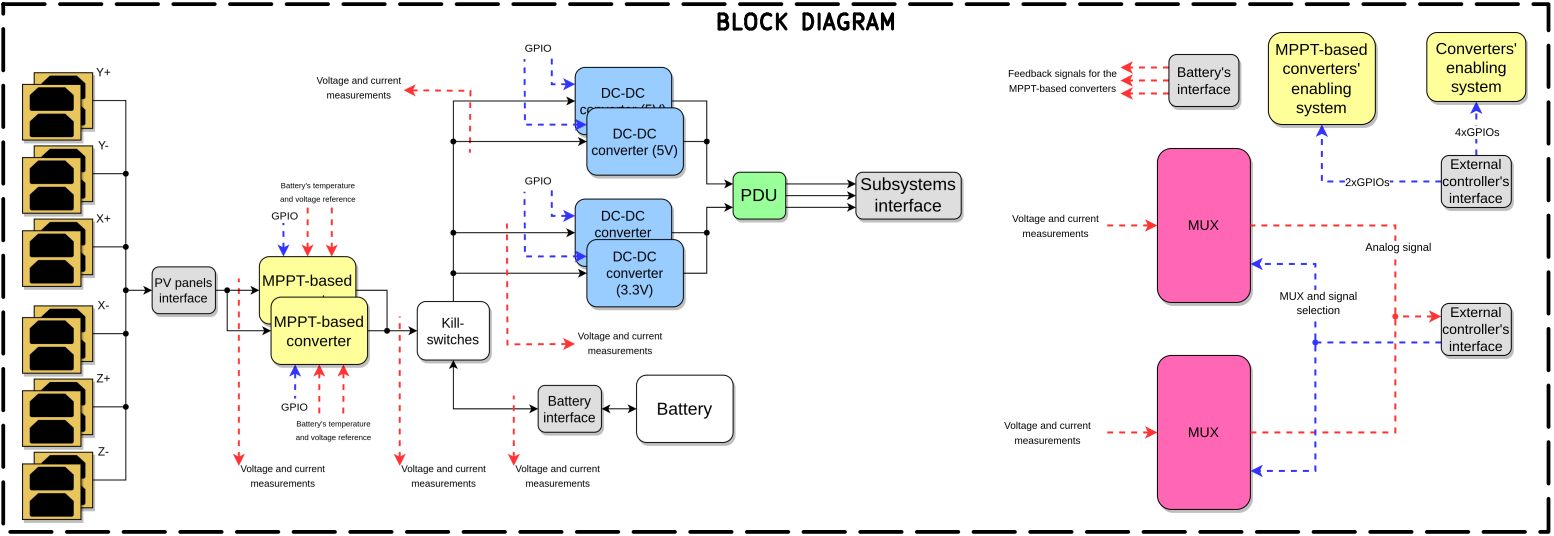
\includegraphics[width=\textwidth, keepaspectratio]{images/reeps-block-diagram.png}
    \end{center}
    \fonte{\textcite{reeps-doc}.}
    \label{fig:reeps-diagrama-blocos}
\end{figure}

Este módulo possui sistema de distribuição centralizado, sistema de harvesting co \gls{PPT}, múltiplos estágios de conversão e barramento principal não regulado.
Possui redundâncias em hardware nos principais subsistemas e não utiliza microcontrolador, visando aumentar a robustês à radiação.

O sistema de harvesting consiste em um barramento com dois \gls{BCR}s BQ24650, configurados em redundância fria, para realização de \gls{MPPT} e sensores de corrente e tensão na entrada e saída dos reguladores.

O sistema de armazenamento, similarmente ao \gls{EPS2}, utilizará um módulo de baterias dedicado, atualmente em estágio inicial de desenvolvimento.
\red{Confirmar!!}

O sistema de distribuição é composto por dois barramentos regulados, de 3.3V e 5V, seis canais de saída controlados individualmente e sensores de tensão e corrente em diversos pontos.
Cada barramento utiliza dois reguladores LTC3833 configurados em redundância fria e sensor de tensão à saída do regulador. Os canais de saída possui também sensores de corrente individuais para monitoramento.

Os sinais de todos os sensores podem ser acessados e lidos através de um multiplexador analógico presente no \gls{EPS}.



% ----------------------------------------------------------

\subsection{Considerações}\label{sec:consideracoes-arq-top}

Observando as topologias e arquiteturas de diferentes projetos, pode-se identificar uma série de características comumente presentes no design de um módulo EPS e relevantes para a etapa de testes:

\begin{itemize}
    \item Multiplos estágios de conversão;
    \begin{itemize}
        \item Reguladores para \gls{MPPT}; % Interface com painéis solares
        \item Reguladores para bateria (\gls{BCR});
        \item Reguladores para os barramentos de saída;
    \end{itemize}
    \item Controle dos barramentos (chaves de potência);
    \item Circuitos de proteção;
    \begin{itemize}
        \item Proteção dos barramentos;
        \item Proteção das baterias;
    \end{itemize}
    \item Aquecimento de baterias;
    \item Monitoramento;
    \begin{itemize}
        \item Tensão e corrente nos barramentos;
        \item Tensão e corrente nas baterias;
        \item Temperatura das baterias;
    \end{itemize}
    \item Presença de microcontrolador;
    \begin{itemize}
        \item Firmware;
        \item Protocolos de comunicação;
        \item Leitura/escrita de dados;
        \item Funções específicas; % Startup do satélite, modos de energia, modos de operação, proteções emplementadas via software...
    \end{itemize}
\end{itemize}

Evidentemente, um determinado design de \gls{EPS} pode não conter todas estes aspectos simultâneamente, porém, com o intuito de criar um plano de testes destinado a módulos de \gls{EPS} no geral, todos estes apectos serão levados em consideração. Com isso, o mesmo poderá ser aplicado à diferentes módulos, com diferentes arquiteturas, selecionando-se os blocos de teste relevantes para dada arquitetura.


% ----------------------------------------------------------
\section{Campanhas de teste de EPS}\label{sec:testes-epss}
% ----------------------------------------------------------

Além da arquitetura dos módulos, alguns dos trabalhos analisados apresentaram também os testes realizados em seus \gls{EPS}s, que serão apresentados a seguir.

\subsection*{Aalto-2}

No trabalho de \textcite{aalto-eps}, é descrito o planejamnto de testes para o EPS do satélite Aalto-2, assim como são relatados os resultados de testes executados em um modelo protótipo do mesmo.

O planejamento de testes descrito referenciou-se nas orientações do \gls{CDS} e suas filosofias de teste.
No momento da escrita do trabalho de \textcite{aalto-eps}, estavam previstos a fabricação de um modelo de engenharia para ralização de testes funcionais e, posteriormente, a fabricação de um modelo de qualificação ou proto-flight para os testes de qualificação.

Os testes relatados no trabalho foram executados em um modelo protótipo nos estágios iniciais de desenvolvimento, sem o microcontrolador integrado ao módulo. Foram relatados os seguintes testes:

\begin{itemize}
    \item Funcionamento dos conversores DC-DC;
    \item Eficiência do sistema de harvesting (conversores \gls{BCR});
    \item Testes dos circuitos de proteção;
    \item Testes de burn-in;
\end{itemize} 

O funcionamento dos conversores DC-DC foi testado aplicando-se diferentes cargas (incrementalmente até atingirem-se os valores descritos nos requisitos do módulo) à saida e medindo-se tensões e correntes de entrada e saída a fim de obter-se a eficiência. Como os conversores possuem redundância, foram testados tando individualmente quanto em funcioamento paralelo (redundância quente).
Os resultados foram então comparados com os requisitos e também com as informações disponíveis nos datasheets dos conversores, visto que são componentes \gls{COTS}.

O sistema de harvesting foi testado simulando-se o ponto de operação dos painéis solares com fontes de bancada e palicando-se um reostato ao barramento das baterias. Foram medidas tensões e correntes à entrada e saída dos conversores \gls{BCR} utilizados para realizar \gls{MPPT} a fim de obter-se a eficiência.
Os resultados foram então comparados com os requisitos.

Para proteção contra over-current é utilizado o componente MAX890L. Sua operação foi testada aplicando-se passagem de corrente ao componente de forma incremental até que o limite imposto fosse atingido.

O teste de burn-in consistiu em aplicar uma alta demanda de potência ao EPS por um longo período de tempo.
Foram aplicadas cargas de 4.5W e 2.5W aos conversores de 5V e 3.3V, respectivamente, por um período de 7 dias. Após o teste, as características da placa foram medidas e comparadas com resultados anteriores.

\subsection*{ESTCube-1}

No artigo de \textcite{estcube-eps} são relatados os testes realizados para qualificação do \gls{EPS} do satélite ESTCube-1. A filosofia de testes adotada foi de \textit{proto-flight testing}, ou seja, o mesmo módulo utilizado nos testes de qualificação foi utilizado como modelo de vôo.
Um modelo de engenharia testes funcionais e de desenvolvimento, porém estes não foram descritos detalhadamente no artigo.

Foram relatados os seguintes testes:
\begin{itemize}
    \item Vibração senoidal e aleatória;
    \item Choque mecânico;
    \item Ciclagem térmica;
    \item Termo vácuo;
\end{itemize}

Além disso, foram realiazdos testes de estresse dos principais componentes do módulo antes da montagem do \gls{EPS}, incluíndo testes de ciclagem térmica, ciclagem de carga e em vácuo das baterias utilizadas.

Foram medidas também a eficiência dos conversores utilizados, para diferentes tensões de entrada e diferentes cargas.


\subsection*{MIST}

O trabalho de \textcite{mist-eps} descreve em detalhe os procedimentos de testes funcionais realizados no \gls{EPS} do satélite MIST.
Neste CubeSat, foram empregados módulos comerciais para toda a plataforma de serviço, inclusive para o \gls{EPS}, utilizando o modelo NanoPower P31u \cite{p31u-datasheet} em conjunto com a placa de baterias BP4 \cite{bp4-datasheet}, ambos fabricados pela GomSpace.

Os principais objetivos destes testes funcionais eram: verificar a análise de power budget, medir o \gls{DoD} das baterias e verificar que a demanda de potência das cargas úteis não interfere no funcionamento do \gls{EPS}.

Para a execução dos testes, foi desenvolvida uma plataforma de testes constituida por uma plataforma flat-sat, simuladores de paineis solares e simuladores de consumo das cargas úteis, todos estes desenvolvidos por estudantes que haviam participado do projeto anteriormente.

O planejamento dos testes foi feito seguindo as orientações da \gls{ECSS} para testes \cite{ecss-e-st-10-03}.
Os testes foram divididos em blocos, sendo o primeiro bloco com testes funcionais e os outros cinco blocos com testes de missão, simulando o consumo e tempo de acionamento de diferentes cargas úteis do satélite de acordo com a operação esperada.

A seguir estão listados, resumidamente, os principais testes executados no \gls{EPS} do satélite MIST, assim como as medidas realizadas em cada teste:

\begin{itemize}
    \item Funcionais:
    \begin{itemize}
        \item Proteção de overcurrent dos barramentos;
        \item Proteção contra overcharge e overdischarge das baterias;
    \end{itemize}
    \item Nenhuma payload ligada:
    \begin{itemize}
        \item Cenários de melhor e pior caso;
        \item Medidas de consumo do sistema, potência dos painéis, tensão e temperatura da bateria em cada cenário;
    \end{itemize}
    \item Combinações de payloads ligadas:
    \begin{itemize}
        \item Cenários de melhor e pior caso;
        \item Medida de tensão e temperatura da bateria;
        \item Medida da potência de saída dos barramentos;
    \end{itemize}
    \item Fast Charge/Discharge da bateria:
    \begin{itemize}
        \item Usado como referência do carregamento e descarregamento da bateria com as condições maximas suportadas pelo EPS;
        \item Não é um cenário esperado durante a operação;
        % \item Mediram apenas a variação da tensão nas baterias, não levaram em conta a corrente para o acumulo de carga mais preciso;
    \end{itemize}
\end{itemize}



\subsection*{EPS 2.0}

Encontra-se na documentação do \gls{EPS2} \cite{eps2-doc} um capítulo descrevendo os procedimentos de teste a serem executados no módulo.
Tem-se também documentados relatórios de testes feitos em modelos de engenharia deste \gls{EPS}.

A documentação para a missão GOLDS-UFSC \cite{golds-ufsc-doc}, na qual será utilizado este \gls{EPS}, apresenta-se uma matriz de testes base a ser adaptada e executada para cada um dos módulos que compõem o satélite.
Para cada módulo, testes mais específicos poderão ser acrescentados à matriz base, que é mostrada na \autoref{tab:matriz-testes-golds}.
Os tests foram organizados em blocos, envolvendo uma série de inspeções, testes elétricos, funcionais.

\begin{table}[htp]
    \centering
    \caption{Matriz de testes do EPS 2.0.}
    \begin{tabular}{l|p{105mm}|p{5mm}}
        \toprule[1.5pt]
        Test type     & Subtests & ID \\
        \midrule
        A. Visual Inspection     & 1. Packaging quality assessment \newline 2. Board manufacturing and assembly quality \newline 3. 3D model comparison \newline 4. Layers marker \newline 5. Labels (schematics comparison) \newline 6. High resolution photos for documentation & TA1 \newline TA2 \newline TA3 \newline TA4 \newline TA5 \newline TA6 \\
        \midrule
        B. Mechanical Inspection     & 1. Board dimensions and mounting holes positioning \newline 2. Board weight measurement & TB1 \newline TB2 \\
        \midrule
        C. Integration Inspection    & 1. Check connectors pinout against the documentation \newline 2. Check connectors positioning & TC1 \newline TC2 \\
        \midrule
        D. Electrical Inspection     & 1. Solder shorts \newline 2. Missing components \newline 3. Lifted pins \newline 4. Poor soldering \newline 5. Swapped components \newline 6. Components partnumber & TD1 \newline TD2 \newline TD3 \newline TD4 \newline TD5 \newline TD6 \\
        \midrule
        E. Electrical Testing       & 1. Continuity test \newline 2. Power up procedures \newline 3. Average input power consumption measurement \newline 4. Average output power source measurement \newline 5. Power tracks temperature \newline 6. Simple signal integrity & TE1 \newline TE2 \newline TE3 \newline TE4 \newline TE5 \newline TE6 \\
        \midrule
        F. Functional Testing     & 1. Simple test code run \newline 2. System code run \newline 3. System hardware self-test flags check \newline 4. Monitor LEDs behavior \newline 5. Monitor the debug serial port logs & TF1 \newline TF2 \newline TF3 \newline TF4 \newline TF5 \\
         \midrule
        G. Module Testing     & 1. Review operation behavior \newline 2. Review features and requirements fulfillment \newline 3. Review communication buses configuration and protocol \newline 4. Review data packages, power buses, and control signals \newline 5. Review edge cases and evaluate damage \newline 6. Run remote automated code tests \newline 7. Run system test codes in the board \newline 8. Run latest stable code version and review behavior & TG1 \newline TG2 \newline TG3 \newline TG4 \newline TG5 \newline TG6 \newline TG7 \newline TG8  \\
        \bottomrule[1.5pt]
    \end{tabular}
    \fonte{\textcite{golds-ufsc-doc}.}
    \label{tab:matriz-testes-golds}
\end{table}

As inspeções e testes descritos acima foram executados no modelo de engenharia do \gls{EPS2}, além disso, testes funcionais adicionais foram acrescentados e executados. Os resultados detalhados encontram-se no relatório presente nos Apêndices A e B da documentação do \gls{EPS2} \cite{eps2-doc}. Observando-se estes relatórios, identificam-se os seguintes testes:

\begin{itemize}
    \item Inspeções:
    \begin{itemize}
        \item Visual;
        \item Mecânica;
        \item Elétrica;
        \item De integração;
    \end{itemize}
    \item Testes elétricos:
    \begin{itemize}
        \item Teste dos conversores;
    \end{itemize}
    \item Testes funcionais:
    \begin{itemize}
        \item Gravação do firmware;
        \item Barramentos de comunicação;
        \item Leitura dos sensores;
        \item Funcionamento do monitor de baterias (DS2777G+);
        \item Controle dos aquecedores de bateria;
        \item Funcionamento do algorítimo de \gls{MPPT};
    \end{itemize}
\end{itemize}

Para todos os testes, o \gls{EPS} foi alimentado por uma fonte de bancada, através de uma flatsat.

As inspeções visam verificar a qualidade do processo de fabricação, conformidade com os arquivos de projeto e integridade mecânica e elétrica do módulo.

Os testes dos conversores foram realiazdos aplicando-se diferentes cargas à saída de cada barramento do \gls{EPS}, avaliando-se a ocorrencia de quedas de tensão ou outras anomalias.

A versão mais recente do firmware foi gravada ao MSP430 e o funcionamento foi aferido através dos logs enviados ao computador via \gls{UART}.

Os principais barramentos de comunicação, com o \gls{OBDH} via \gls{I2C} e com o \gls{TTC} via \gls{UART}, foram testados utilizando-se um analizador lógico e verificando a integridade dos pacotes enviados.

A leitura dos sensores foi verificada comparando-se as medidas reportadas nos logs do \gls{EPS} com medidas realizadas por instrumentos de medição externos.

O funcionamento do monitor de baterias foi verificado através da leitura dos registradores internos do CI, comparando-se com os valores e configurações esperados.

Para o teste do controle dos aquecedores de bateria, seus limiares máximo e mínimo de temperatura foram alterados para valores acima da temperatura ambiente (32°C e 26°C, respectivamente), e as leituras dos sensores de temperatura foram monitoradas durante um período de tempo.

O algorítimo de \gls{PO} para o \gls{MPPT} foi testado com testes unitários no firmware.
O sinal de \gls{PWM} gerado pelo micorcontrolador e utilizado para controle dos conversore boost que realizam o \gls{MPPT} foi avaliado utilizando-se um osciloscópio.